\chapter{实验设计及结果分析}\label{chap:Result}

本章节主要介绍基于前述算法设计的LS\_NRA求解工具的实验结果,并基于此对其性能进行了分析。本章节主要可以分为三个部分:首先我们介绍实验安排和实验条件,包括测试样例、比较方法、运行环境等;然后我们给出LS\_NRA与其他主流求解器的求解个数与时间对比;最后我们对前述算法进行了消融实验,确保本文介绍的算法的有效性。

\section{实验设置}
\textbf{实验样例:} 本工作选取SMT-LIB中QF\_NRA理论作为测试样例。测试样例大多包含来自工业问题的实例,如非线性混成自动机的分析(hycomp),程序终止验证的秩函数生成(LassoRanker)等。Kissing样例则包含了球体吻合问题,即给定一个维度,最多可以有多少个一样的球可以和给定的球相切,并且保证两两之间不相交。通过SMT求解器的计算,每一个测试样例会被返回可满足(sat),不可满足(unsat)或者未知(unknown)。在实际测试中,很多标注为未知的问题往往被其他的求解器(Z3、cvc5)证明为不可满足。由于局部搜索往往用于计算可满足问题,因此在实际测试中,我们首先从SMT-LIB中选择标注为可满足或未知的样例,然后剔除掉被其他求解器证明为不可满足的部分。SMT-LIB包含了各种不同难度的样例,但是并没有显著标注难度等级。比如,metitarski里面的一些样例(来自于MetiTarski工具)一般只包含很少的约束,对局部搜索和完备算法均不构成挑战。最终,我们收集了6216个测试样例。


\textbf{实验环境:} 所有实验都在一台配备有Intel Xeon Platinum 8153(2.00GHz)和2048G RAM 的服务器上进行,系统为Centos 7.7.1908。每一个样例设置的时间限制为20分钟(和SMT比赛相同),内存限制为30GB。

\section{LS\_NRA求解NRA样例的能力}
我们在表\ref{tab:experiment}中展示了我们的工具LS\_NRA与其他主流SMT求解器的性能对比。我们的工具一个主要优势是针对Sturm-MBO样例,一种只包含一个非常复杂度数很高的多项式的约束。目前主流的完备算法在该问题上没有求解成功。我们的工具在其他样例上表现也很突出,基本可以和主流求解器的效果持平。

除此之外,我们的算法和Z3、cvc5有很大的互补性。根据表\ref{tab:experiment},一共有来自不同类别共148个样例仅仅可以使用局部搜索算法求解,而非Z3、cvc5、Yices等完备算法。更具体来说,有291个样例可以被局部搜索求解而非Z3,有378个样例可以被局部搜索求解而非cvc5。

\begin{table*}[]
    \centering
    \resizebox{\linewidth}{!}{
        \begin{tabular}{c | c | c | c | c | c | c}
            \hline
            类别 & 个数 & Z3 & cvc5 & Yices & LS\_NRA (本文) & 单独求解 \\\hline
            20161105-Sturm-MBO & 120 & 0 & 0 & 0 & 88 & 88 \\
            20161105-Sturm-MGC & 2 & 2 & 0 & 0 & 0 & 0 \\
            20170501-Heizmann & 60 & 3 & 1 & 0 & 8 & 6 \\
            20180501-Economics-Mulligan & 93 & 93 & 89 & 91 & 90 & 0 \\
            2019-ezsmt & 61 & 54 & 51 & 52 & 19 & 0 \\
            20209011-Pine & 237 & 235 & 201 & 235 & 224 & 0 \\
            20211101-Geogebra & 112 & 109 & 91 & 99 & 101 & 0 \\
            20220314-Uncu & 74 & 73 & 66 & 74 & 70 & 0 \\
            LassoRanker & 351 & 155 & 304 & 122 & 272 & 13 \\
            UltimateAtomizer & 48 & 41 & 34 & 39 & 27 & 2 \\
            hycomp & 492 & 311 & 216 & 227 & 304 & 11 \\
            kissing & 42 & 33 & 17 & 10 & 33 & 1 \\
            meti-tarski & 4391 & 4391 & 4345 & 4369 & 4351 & 0 \\
            zankl & 133 & 70 & 61 & 58 & 100 & 27 \\\hline
            总和 & 6216 & 5570 & 5476 & 5376 & 5687 & 148 \\\hline
        \end{tabular}
        }
        \bicaption{LS\_NRA和其他SMT求解器的求解能力对比。} {Comparison of LS\_NRA and other SMT solvers.}
\label{tab:experiment}
\end{table*}

我们在图\ref{fig:scatter}中描绘了LS\_NRA与Z3、cvc5求解时间对比的散点图。图中每一个点的横坐标代表了求解该样例LS\_NRA所需要的时间,纵坐标表示了其他求解器的求解时间,虚线则说明二者在该问题上消耗的求解时间一致。我们注意到在SMT-LIB测试样例中存在大量相对简单的问题。为了考虑这些问题的因素,我们统计了Z3、cvc5和LS\_NRA在1秒内解决的问题个数,共计4765个,这样仅仅剩下1451个被认为是难以求解的样例。从这点来看,LS\_NRA在求解总数、单独求解和互补性上均有优势。

\begin{figure*}[t]
    \centering
    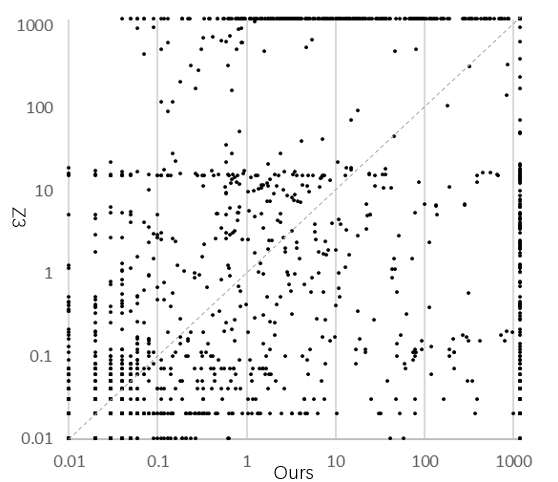
\includegraphics[width=0.45\columnwidth]{Img/scatter_z3b.png}\qquad
    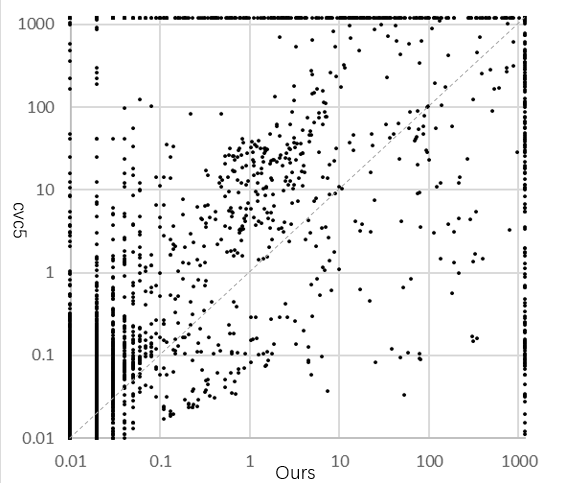
\includegraphics[width=0.45\columnwidth]{Img/scatter_cvc5b.png}
    \bicaption{LS\_NRA与Z3、cvc5求解时间对比。}{Comparison of LS\_NRA and Z3, cvc5 solving time.}
\label{fig:scatter}
\end{figure*}

\section{和其他局部搜索工作的对比}
我们还讨论了LS\_NRA与以往局部搜索工作的对比。在\cite{multilinear}考虑的979个多线性样例中,LS\_NRA可以求解826个,略小于前序工作的891个。这种微弱的差异主要来自于\cite{multilinear}更高效的实现,考虑到其工作进需要考虑有理数赋值,而非代数数,因此在数据结构设计和参数优化上更有针对性。在\cite{LiXZ23}考虑的2736个样例中,我们的方法可以求解2589个,高于前序工作的2246个。事实上,我们不仅比局部搜索算法求解的个数要多,也要比前面工作用于对比的其他求解器个数还要多。我们注意到\cite{LiXZ23}使用了不同的计算软件(比如Maple),并且在不同机器上测试,因此数据可能略有误差。

\section{消融实验1:变量分数增量式计算的影响}
本小节主要展示章节\ref{chap:method1}中提出的变量分数增量式计算对迭代加速的影响。我们比较如下集中实现:基于边界的增量式计算(Incremental),不采用增量式计算的传统方法(Naive),以及传统方法但是限制每次考虑的子句数最大为45(Limit-45)。相关的结果如表格\ref{tab:incremental}所示。

我们注意到不同实现方法的求解总数差异并不大,并且主要集中在LassoRanker类别上。LassoRanker样例一般需要比较长时间求解,因此不同实现方法对迭代速度的影响十分重要。通过对比求解时间可以看出对于一个特定的问题而言,Naive和Limit-45的方法基本需要消耗2-10倍于Incremental方法的时间,具体的倍数在不同问题上有所不同。对于限制时间为20分钟的实验,总数的差异并不大,但是这种差异会随着限制时间的减小而增大,特别是当局部搜索融入到其他方法中使用时。

\begin{table*}[]
    \centering
    \resizebox{\linewidth}{!}{
        \begin{tabular}{c | c | c | c | c}
            \hline
            类别 & 个数 & Incremental & Naive & Limit-45 \\\hline
            20161105-Sturm-MBO & 120 & 88 & 85 & 85 \\\hline
            20161105-Sturm-MGC & 2 & 0 & 0 & 0 \\\hline
            20170501-Heizmann & 60 & 8 & 5 & 5 \\\hline
            20180501-Economics-Mulligan & 93 & 90 & 89 & 89 \\\hline
            2019-ezsmt & 61 & 19 & 19 & 15 \\\hline
            20209011-Pine & 237 & 224 & 222 & 222 \\\hline
            20211101-Geogebra & 112 & 101 & 101 & 101 \\\hline
            20220314-Uncu & 74 & 70 & 70 & 70 \\\hline
            LassoRanker & 351 & 272 & 264 & 269 \\\hline
            UltimateAtomizer & 48 & 27 & 26 & 26 \\\hline
            hycomp & 492 & 304 & 298 & 298 \\\hline
            kissing & 42 & 33 & 32 & 33 \\\hline
            meti-tarski & 4391 & 4351 & 4352 & 4352 \\\hline
            zankl & 133 & 100 & 100 & 100 \\\hline
            总和 & 6216 & 5687 & 5663 & 5665 \\\hline
        \end{tabular}
        }
        \bicaption{增量式计算对算法的影响。} {Impact of incremental calculation on algorithm.}
\label{tab:incremental}
\end{table*}

\section{消融实验2:等式约束松弛的影响}
本小节主要展示章节\ref{chap:method2}中介绍的等式约束松弛对整体算法的影响。我们给出以下三种版本:使用等式松弛机制(Relaxation),不适用等式松弛但优先选取低复杂度的赋值(Threshold),不使用等式松弛并且不考虑赋值复杂度(NoOrder)。相关结果在表\ref{tab:relaxation}中展示。

试验结果表明,当把赋值复杂度考虑在内时可以保证对于大多数类别提升求解能力。

\begin{table*}[]
    \centering
    \resizebox{\linewidth}{!}{
        \begin{tabular}{c | c | c | c | c}
            \hline
            类别 & 个数 & Relaxation & Threshold & NoOrder \\\hline
            20161105-Sturm-MBO & 120 & 88 & 100 & 99 \\\hline
            20161105-Sturm-MGC & 2 & 0 & 0 & 0 \\\hline
            20170501-Heizmann & 60 & 8 & 9 & 3 \\\hline
            20180501-Economics-Mulligan & 93 & 90 & 89 & 86 \\\hline
            2019-ezsmt & 61 & 19 & 19 & 19 \\\hline
            20209011-Pine & 237 & 224 & 223 & 222 \\\hline
            20211101-Geogebra & 112 & 101 & 98 & 92 \\\hline
            20220314-Uncu & 74 & 70 & 70 & 70 \\\hline
            LassoRanker & 351 & 272 & 277 & 278 \\\hline
            UltimateAtomizer & 48 & 27 & 26 & 20 \\\hline
            hycomp & 492 & 304 & 211 & 164 \\\hline
            kissing & 42 & 33 & 31 & 27 \\\hline
            meti-tarski & 4391 & 4351 & 4353 & 4360 \\\hline
            zankl & 133 & 100 & 100 & 100 \\\hline
            总和 & 6216 & 5687 & 5606 & 5540 \\\hline
        \end{tabular}
        }
        \bicaption{等式约束松弛对算法的影响。} {Impact of relaxation on algorithm.}
\label{tab:relaxation}
\end{table*}
